{\Large The SIGDIAL organizers gratefully acknowledge the support from the following sponsors.}
\bigskip

\vspace*{1cm}

\vspace*{1cm}
\noindent
{\Large \textbf{Gold}}\\\\

\includegraphics[width=2cm]{sponsor_logos/apple.png}\hfill
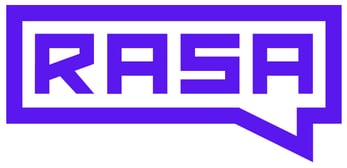
\includegraphics[width=2cm]{sponsor_logos/rasa.jpg}\hfill
\vspace*{1cm}

\vspace*{1cm}
\noindent
{\Large \textbf{Silver}}\\\\
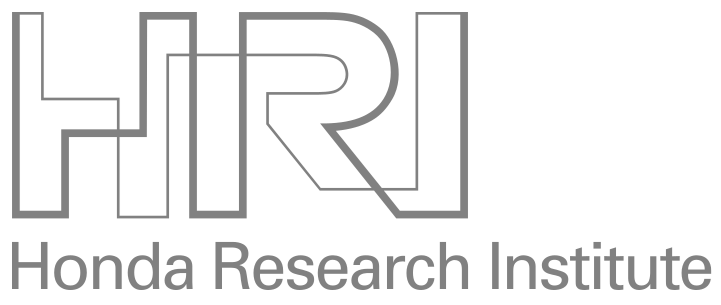
\includegraphics[width=2cm]{sponsor_logos/honda.png}\hfill

\includegraphics[width=2cm]{sponsor_logos/toshiba.jpeg}\hfill
\vspace*{1cm}

\vspace*{1cm}
\noindent
{\Large \textbf{In cooperation with:}}\\\\

\includegraphics[width=2cm]{sponsor_logos/boise.png}\hfill
\vspace*{1cm}

\newpage

\begin{center}
\Large \textbf{Introduction}\\
\end{center}
We are excited to welcome you to SIGDIAL 2020, the 21st Annual Meeting of the Special Interest Group on Discourse and Dialogue. This year the conference is being held virtually, on July 1-3, 2020, with the Satellite Event YRRSDS 2020 (Young Researchers' Roundtable on Spoken Dialog Systems) and just before ACL 2020 that will take place also virtually July 5-10, 2020.  

The SIGDIAL conference is a premier publication venue for research in discourse and dialogue. This year, the program includes three keynote talks, nine presentation sessions, three demo sessions, and a special session entitled ``Situated Dialogue with Virtual Agents and Robots (RoboDial 2.0)'' organized by Jose David Lopes, Stephanie Lukin, Matthew Marge, Vikram Ramanarayanan,  Matthias Scheutz, Casey Kennington, and Cynthia Matuszek.

We received 104 submissions this year, which comprised 62 long papers, 32 short papers and 10 demo descriptions. This year, for the first time, we had 8 Senior Program Committee (SPC) members who were responsible for a set of 10-15 papers each, guiding the discussion process and writing a meta-review. Every submission was assigned to one SPC and received at least three reviews. When making our selections for the program, we carefully considered the reviews, meta-reviews and the comments made during the discussions among reviewers. The members of the Senior Program Committee and Program Committee did an excellent job in reviewing the submitted papers, and we thank them for their essential role in selecting the accepted papers and helping produce a high quality program for the conference. In line with the SIGDIAL tradition, our aim has been to create a balanced program that accommodates as many favorably rated papers as possible. We accepted 41 papers: 23 long papers, 10 short papers, and 8 demo descriptions. These numbers give an overall acceptance rate of 39\%. The acceptance rate for long papers (37\%) and short papers (31\%) remains in line with the acceptance rate from last year.

Each of the three conference days features one keynote and several oral sessions, with the remaining time given to demos, special session and sponsor sessions. In organizing the virtual conference, we decided to keep as much as possible the spirit of an in person conference. All keynotes, talks and demos are pre-recorded and made available at the beginning of the conference for participants to watch asynchronously. The long and short papers are organized in thematic sessions and take into consideration the speakers' different time zones.  The sessions contain 3-4 pre-recorded talks followed by a Live QA part with the presenters. For demos, we organized Live Question Answering sessions with the demo presenters. Topic-wise, we have papers on evaluation and corpora, natural language generation, task oriented dialogues, knowledge use and acquisition,  behaviour modeling, dialogue policy and dialogue state tracking, modeling convergence in dialogues, and the semantics and pragmatics of discourse and dialogue. 

A conference of this scale requires advice, help and enthusiastic participation of many parties, and we have a big `thank you' to say to all of them. Regarding the program, we thank our three keynote speakers, Asli Celikyilmaz (Microsoft Research), Diane Litman (University of Pittsburgh) and Gabriel Skantze (KTH Royal Institute of Technologies),   for their inspiring talks on "Neural text Generation: Progress and Challenges", "Argument Mining, Discourse Analysis, and Educational Applications" and "Conversational Turn-taking in Human-robot Interaction". 
%SM need to wait for title of invited speakers 
We also thank the organizers of the special session on Situated Dialogue with Virtual Agents and Robots (RoboDial 2.0). We are grateful for their smooth and efficient coordination with the main conference.

%SM need to thank also virtual presentation chairs
We extend special thanks to our Local Chair, Casey Kennington, for handling the  situation of adapting to a virtual conference. SIGDIAL 2020 would not have been possible without his effort in arranging the virtual platform, handling registration, numerous preparations for the conference, and last but not least, Casey's personal contributions, which exceeded those of a local organizer. We also thank the virtual presentation co-chairs, Koji Inoue and Erik Ekstedt, for helping the authors with their video presentations, arranging for the video streaming during the conference and hosting the Zoom Live QAs sessions. 

David Vandyke, our Sponsorship Chair, has conducted the massive task of recruiting and liaising with our conference sponsors, many of whom continue to contribute year after year. We thank David for his dedicated work and his assistance with conference planning. We gratefully acknowledge the support of our sponsors: (Gold level) Apple and Rasa Technologies and (Silver level) Toshiba Research Europe and Honda Research Institute. %We also thank the Boise State University for its generous sponsorship as host. (I am not sure whether we should include the host or not given our virtual conference plan.)

In addition, we thank Nina Dethlefs, Mentoring Chair for SIGDIAL 2020, for her dedicated work on the mentoring process. The goal of mentoring is to assist authors of papers that contain important ideas but require significant stylistic modifications, and we thank our mentoring team for their excellent support of the authors; and Stefan Ultes, our publication chair, capped the long organizational process by putting together these high quality conference proceedings.

We thank the SIGdial board, both current and emeritus officers, Gabriel Skantze, Mikio Nakano, Vikram Ramanarayanan, Ethan Selfridge, Jason Williams and Amanda Stent, for their advice and support from beginning to end.

We once again thank our senior program committee members (Dilek Hakkani-Tur,    Annie Louis, Mikio Nakano, Rebecca J. Passonneau, Gabriel Skantze,  Manfred Stede, David Traum, Koichiro Yoshino) and program committee members for committing their time to help us select an excellent technical program. Finally, we thank all the authors who submitted to the conference and all conference participants for making SIGDIAL 2020 a success and for growing the research areas of discourse and dialogue with their fine work.

\vspace*{2cm}

Olivier Pietquin, General Chair

Smaranda Muresan and Yun-Nung (Vivian) Chen, Program Co-Chairs
